\documentclass[]{compositionalityarticle}

\title{A Compositional Framework for Reaction Networks}

\author[1,2]{John C. Baez}
\author[3]{Blake S. Pollard}

\affil[1]{Department of Mathematics University of California Riverside CA, USA 92521}
\affil[2]{Centre for Quantum Technologies National University of Singapore, Singapore 117543}
\affil[3]{Department of Physics and Astronomy University of California, Riverside CA 92521}

\dates{May 19, 2017}

\leadauthor{Beaz}

\email{baez@math.ucr.edu}
\email{bpoll002@ucr.edu}

\begin{abstract}
Reaction networks, or equivalently Petri nets, are a general framework
for describing processes in which entities of various kinds interact and
turn into other entities. In chemistry, where the reactions are assigned
‘rate constants’, any reaction network gives rise to a nonlinear dynamical
system called its ‘rate equation’. Here we generalize these ideas to ‘open’
reaction networks, which allow entities to flow in and out at certain designated
inputs and outputs. We treat open reaction networks as morphisms
in a category. Composing two such morphisms connects the outputs of
the first to the inputs of the second. We construct a functor sending
any open reaction network to its corresponding ‘open dynamical system’.
This provides a compositional framework for studying the dynamics of
reaction networks. We then turn to statics: that is, steady state solutions
of open dynamical systems. We construct a ‘black-boxing’ functor that
sends any open dynamical system to the relation that it imposes between
input and output variables in steady states. This extends our earlier work
on black-boxing for Markov processes.
\end{abstract}

\begin{document}

\maketitle
\twocolumn
\abstractcontent
\merriweatherlight

\section{Introduction}
Reaction networks, first formally defined by Aris \cite{2004quant.ph..2130A} in 1965, are a framework
for describing processes whereby entities interact and transform into other entities.
While they first arose in chemistry, and are often called ‘chemical reaction
networks’, their applications are widespread. For example, a basic model of
infectious disease, the SIRS model, is described by this reaction network:

\begin{equation*} 
  S + I \xrightarrow{\iota} 2 I
  I \xrightarrow{\rho} R \xrightarrow{\lambda} S 
\end{equation*}

We see here three types of entity, called ‘species’:
\begin{itemize}
  \item S: \textbf{susceptible},
  \item I: \textbf{infected},
  \item R: \textbf{resistant}.
\end{itemize}
We also have three ‘reactions’:
\begin{itemize}
  \item $\iota$: $S + I \rightarrow 2I$: \textbf{infection}, in which a susceptible individual meets an
infected one and becomes infected;
  \item $\rho$: $I \rightarrow R$: \textbf{recovery}, in which an infected individual gains resistance to
the disease;
  \item $\lambda$: $R \rightarrow S$: \textbf{loss of resistance}, in which a resistant individual becomes
susceptible.
\end{itemize}
In general, a reaction network involves a finite set of species, but reactions go
between ‘complexes’, which are finite linear combinations of these species with
natural number coefficients. The reaction network is a directed graph whose
vertices are certain complexes and whose edges are called ‘reactions’.
If we attach a positive real number called a ‘rate constant’ to each reaction,
a reaction network determines a system of differential equations saying how the
concentrations of the species change over time. This system of equations is
usually called the ‘rate equation’. In the example above, the rate equation is

\begin{multline}
  \frac{dS}{dt} = r_{\lambda} R - r_{\iota} SI \\
  \frac{dI}{dt} = r_{\iota} SI - r_{\rho} I \\
  \frac{dR}{dt} = r_{\rho} I - r_{\lambda} R
\end{multline}

Here $r_{\iota}$, $r_{\rho}$ and $r_{\lambda}$ are the rate constants for the three reactions, and $S$, $I$, $R$
now stand for the concentrations of the three species, which are treated in a
continuum approximation as smooth functions $S, I, R: \mathbb{R} \rightarrow [0, \infty)$. The rate
equation can be derived from the ‘law of mass action’, which says that any
reaction occurs at a rate equal to its rate constant times the product of the
concentrations of the species entering it as inputs.
A reaction network is more than just a stepping-stone to its rate equation.
Interesting qualitative properties of the rate equation, such as existence and
uniqueness of steady state solutions, can often be determined simply by examining
the reaction network, independent of any particular choice of rate constants.
Results in this direction began with Feinberg and Horn’s seminal work in the
1960’s \cite{2015arXiv150405625B, 2015arXiv151200802S}, leading to the Deficiency Zero and Deficiency One Theorems
\cite{2016arXiv160508100C, 2016arXiv160905382F}  and more recently to a proof of the Global Attractor Conjecture [11].
In this paper we present a ‘compositional framework’ for reaction networks:
that is, a way to build up a reaction network from smaller pieces, in such a way
that its rate equation can be determined from those of the pieces. However,
this framework requires that we view reaction networks in a somewhat different
way, as ‘Petri nets’.

Petri nets were invented by Carl Petri in 1939, when he was just a teenager,
for the purposes of chemistry [32]. Much later, they became popular in theoretical
computer science [23, 31], biology [26, 27, 36], and other fields [3, 22, 29].
A Petri net is a bipartite directed graph; vertices of one kind represent species,
while those of the other kind represent reactions. The edges into a transition
specify which species are inputs to that transition, while the edges out specify
its outputs. One can easily turn a reaction network into a Petri net and vice
versa. For example, the reaction network above translates into this Petri net:

\begin{figure}
  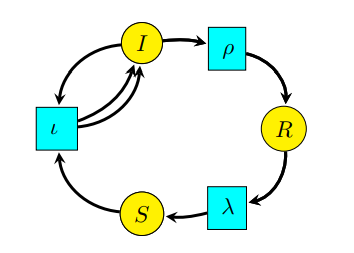
\includegraphics[width=0.5 \textwidth]{fig1.png}
\end{figure}


One should beware that the terminology is diverse, since it comes from several
communities. In the Petri net literature, species are called ‘places’ and reactions
are called ‘transitions’. Indeed, Petri nets are sometimes called ‘place-transition
nets’ or ‘P/T nets’. On the other hand, chemists call them ‘species-reaction
graphs’ or ‘SR-graphs’. When each reaction of a Petri net has a rate constant
attached to it, it is often called a ‘stochastic Petri net’.

While some qualitative properties of a rate equation can be read off from a
reaction network, others are more easily read from the corresponding Petri net.
For example, properties of a Petri net can be used to determine whether its rate
equation has the capacity to admit multiple steady states [6, 12, 17].

Petri nets are also better suited to a compositional framework. The key new concept required is that of an ‘open’ Petri net. Here is an example:

\begin{figure}
  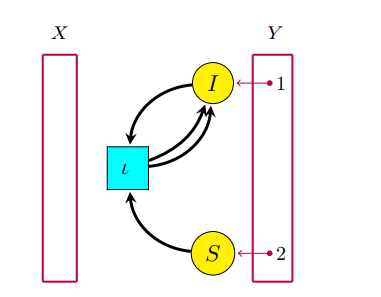
\includegraphics[width=0.5 \textwidth]{fig2.png}
\end{figure}


The box at left shows a set $X$ of ‘inputs’ (which happens to be empty), while
the box at right shows a set $Y$ of ‘outputs’. Both inputs and outputs are points
at which entities of various species can flow in or out of the Petri net. We say
the open Petri net goes from $X$ to $Y$ , and we shall show how to treat it as a
morphism $f : X \rightarrow Y$ in a category we call \texttt{RxNet}.

Given an open Petri net with rate constants assigned to each reaction, we
explain how to systematically obtain its ‘open rate equation’, which amounts to
the usual rate equation with extra terms describing inflows and outflows. The
above example has this open rate equation:


\begin{multline}
  \frac{dS}{dt} = -r_{\iota} SI - o_1 \\
  \frac{dI}{dt} = r_{\iota} I - o_2
\end{multline}

Here $o_1, o_2 : \mathbb{R} \rightarrow \mathbb{R}$ are arbitrary smooth functions describing outflows as a
function of time.
Given another open Petri net $g : Y \rightarrow Z$, for example this:


\section{Reaction networks versus Petri nets}
We begin by precisely defining reaction networks and Petri nets, so we can see
that they are two ways of presenting the same concept.
\begin{definition} A reaction network $(S, T, s, t)$ consists of
%  \begin{imtemize}
  \item a finite set $S$,
  \item a finite set $T$,
  \item functions $s, t: T \rightarrow N^{s}$.
%  \end{itemize}
\end{definition}



\bibliography{compositionality-sample}
\bibliographystyle{plain}
\end{document}


